%! TeX root: ./main.tex
% -*- mode:latex; -*-
\maketitle

Student Name: \hfill Student Email: \hspace{10em}
\section{Instructions}
\begin{itemize}
\item  There are five questions.
\item Maximum number of marks is 120 . This exam
  amounts 10\% toward the final grade.
  \item Time allowed is 50 minutes.
  \item In order to minimize distraction to your fellow students, you may not leave
  during the last 10 minutes of the examination.
  \item The examination is closed-book. One $8\times11$ in two-sided cheatsheet is allowed.
  \item Non-programmable calculators are permitted.
  \item Please use a pen or heavy pencil to ensure legibility. Colored
    pens/pencils are recommended for K-map grouping.
  \item Please show your work; where appropriate, marks will be awarded for proper and well-reasoned explanations.
\end{itemize}

\begin{prob}
A sequential circuit is to be used to control the operation of a vending machine which
dispenses a \$0.25 product. The circuit has three inputs (N, D, and Q) and two outputs
(R and C). The coin detector mechanism in the vending machine is synchronized with the same clock as the sequential circuit you are to design. The coin detector outputs a
single 1 to the N, D, or Q input for every nickel (5 cents), dime (10 cents), or
quarter (25 cents), respectively, that
the customer inserts. Only one input will be 1 at a time. When the customer has
inserted \textit{at least} \$0.25 in any combination of nickels, dimes, and quarters, the vending
machine must give change and dispense the product. The coin return mechanism
gives change by returning nickels to the customer. For every 1 output on C, the coin
return mechanism will return one nickel to the customer. The product is dispensed
when the circuit outputs a single 1 on output R. The circuit should reset after dispensing the product.

\textbf{Example:} The customer inserts a nickel, a dime, and a quarter. The circuit inputs
and outputs could look like this:\\
Inputs:\\
\begin{tabular}{ccccccccccccccccccc}
\multirow{3}*{Inputs} & N=& 0& 0& 0& 1& 0& 0& 0& 0& 0& 0& 0& 0& 0& 0& 0& 0& 0\\
& D=& 0& 0& 0& 0& 0& 0& 0& 1& 0& 0& 0& 0& 0& 0& 0& 0& 0\\
& Q=& 0& 0& 0& 0& 0& 0& 0& 0& 0& 0& 1& 0& 0& 0& 0& 0& 0\\
\multirow{2}*{Outputs}&R=& 0& 0& 0& 0& 0& 0& 0& 0& 0& 0& 0& 0& 0& 0& 1& 0& 0\\
&C=& 0& 0& 0& 0& 0& 0& 0& 0& 0& 0& 0& 1& 1& 1& 0& 0& 0\\
\end{tabular}\\
Note that any number of 0’s can occur between 1 inputs.
Complete the following Moore state table for the sequential circuit, and for each state indicate how much money the customer has inserted or how much change is due. 
\label{p:fsm}
(30 marks)
\end{prob}
% \subsubsection*{Solution}
% \begin{tabular}{p{15mm}p{10mm}cccccp{20mm}}
%   \toprule
%   Money inserted & Change due & PS & \multicolumn{4}{c}{Next State} & Output (RC)\\
%                  &            &  &  NDQ = 000 & NDQ = 100 & NDQ = 010 & NDQ = 001 & \\
%                  \midrule
%   0 & 0 & $S_0$ & $S_0$ & $S_1$ & $S_2$ & $S_3$ & 00 \\
% \end{tabular}

\begin{prob}
  Realize a BCD to excess-3 code converter using a minimum number of gates.
  (The excess-3 code is obtained from the binary numbers (0-9) by adding 3 (0011)
  to each of the binary numbers.)
  (10 marks)
  \label{p:decoder}
\end{prob}

\begin{prob}
  %15.25
  %Do any two of the following three problems (20 marks each):
  %\begin{enumerate}
  %\item 
  Reduce the following state table to a minimum number of states using
  implication charts (20 marks).
  % \item
  % Use the guideline method to determine a suitable state assignment for the
  % reduced table .
  % % \item
  % % Realize the table using D flip-flops.
  % \item
  % Use a random or sequential state assignment to realize the table using J-K
  % flip-flops.
  \\
  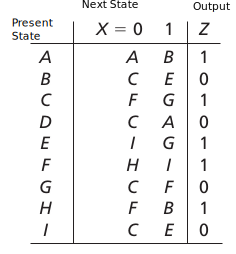
\includegraphics[width=0.3\linewidth]{./media/15.25-state-table.png}
  %\end{enumerate} 
\end{prob}

\begin{prob}
  \begin{enumerate}
    %15.23
  \item For the following state table, use the three guidelines to determine which
  of the three possible nonequivalent state assignments should give the best
  solution (20 marks).
  \item Using your answer to (a), derive J-K flip-flop input equations and the output
  equations (20 marks).\\
  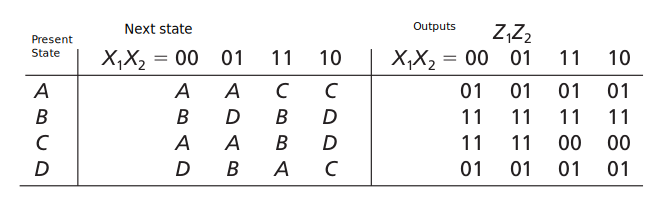
\includegraphics[width=0.5\linewidth]{./media/15.23-state-table.png}
  \end{enumerate}
\end{prob}


% \begin{prob}
%   Use a 4-to-1 multiplexer and a minimum number of external gates to realize the
%   function $F(w, x, y, z) = \sum m(3, 4, 5, 7, 10, 14) + \sum d(1, 6, 15).$
%   The inputs are only available uncomplemented (20 marks).
% \end{prob}
% \newpage
% 
% \begin{prob}
%   % 9 study guide 5
%   The following diagram shows the pattern of 0’s and 1’s stored in a ROM
%   with eight words and four bits per word. What will be the values of $F_1 , F_2 ,
%   F_3 , and F_4$ if $A=0$ and $B = C = 1$?
%   Also give the minterm expansions for $F_1$ and $F_2$ (20 marks).\\
%   \includegraphics[width=0.4\linewidth]{./media/ROM-minterms.png}
% \end{prob}
% \newpage

\begin{prob}
  Find the minimum cost circuit for the following function using K-map. Find both
  sum-of-products and product-of-sum forms and find the minimum cost one.\\
  $ F(a, b, c, d, e) = \prod M(2, 4, 5, 6, 8, 10, 12, 13, 16, 17, 18, 22, 23, 24)
   + \prod
  D(0, 11, 30, 31)$ (20 marks).
\end{prob}
\newpage
